% Homework template for Information Theory and Statistical Learning
% by Xiangxiang Xu <xiangxiangxu.thu@gmail.com>
% LAST UPDATE: Oct 3, 2019
\documentclass[a4paper]{article}
\usepackage[T1]{fontenc}
\usepackage{amsmath, amssymb, amsthm}
% amsmath: equation*, amssymb: mathbb, amsthm: proof
\usepackage{moreenum}
\usepackage{mathtools}
\usepackage{url}
\usepackage{enumitem}
\usepackage{bm}
\usepackage{graphicx}
\usepackage{subcaption}
\usepackage{booktabs} % toprule
\usepackage[mathcal]{eucal}
\usepackage{dsfont}
\usepackage[numbered,framed]{matlab-prettifier}
%% Definitions for Information Theory & Statistical Learning
%% UPDATED: Sep 30, 2019 by Xiangxiang 
\newcommand{\theterm}{Fall 2020}

\newcommand{\thecoursenameshort}{\textsc{Information Theory and Statistical Learning}}
\newcommand{\thecoursename}{
Tsinghua-Berkeley Shenzhen Institute\\
%\vspace*{0.1in}
\thecoursenameshort
}

\newcommand{\courseheader}{
\vspace*{-1in}
\begin{center}
\thecoursename \\
\theterm
\vspace*{0.1in}
\hrule
\end{center}
}
\newcommand{\uc}{\underline{c}}    % c, vec
\newcommand{\uv}{\underline{v}}    % x, vec
\newcommand{\uw}{\underline{w}}    % w, vec
\newcommand{\ux}{\underline{x}}    % x, vec
\newcommand{\uy}{\underline{y}}    % y, vec
\newcommand{\uz}{\underline{z}}    % z, vec
\newcommand{\um}{\underline{m}}    % m, vec
\newcommand{\ut}{\underline{t}}    % t, vec

\newcommand{\bA}{\mathbf{A}}    % A, mat
\newcommand{\bI}{\mathbf{I}}    % A, mat
\newcommand{\bN}{\mathbf{N}}    % n, mat
\newcommand{\bT}{\mathbf{T}}    % T, mat
\newcommand{\bU}{\mathbf{U}}    % U, mat
\newcommand{\bV}{\mathbf{V}}    % V, mat
\newcommand{\bQ}{\mathbf{Q}}    % Q, mat
\newcommand{\bX}{\mathbf{X}}    % X, mat

\newcommand{\bc}{\bm{c}}    % c, vec
\newcommand{\be}{\bm{e}}    % e, vec
\newcommand{\bu}{\bm{u}}    % u, vec
\newcommand{\bv}{\bm{v}}    % v, vec
\newcommand{\bw}{\bm{w}}    % w, vec
\newcommand{\bt}{\bm{t}}    % t, vec
\newcommand{\bx}{\bm{x}}    % x, vec
\newcommand{\by}{\bm{y}}    % y, vec
\newcommand{\bz}{\bm{z}}    % z, vec

\newcommand{\phib}{\bm{\phi}}    % phi, vec
\newcommand{\psib}{\bm{\psi}}    % psi, vec
\newcommand{\dtm}{\mathbf{B}}    %
\newcommand{\dtmt}{\tilde{\dtm}}    %
\newcommand{\Ab}{\mathbf{A}}    % A mat
\newcommand{\Kb}{\mathbf{K}}    % K mat
\newcommand{\Ib}{\mathbf{I}}    % I mat



\newcommand{\rvby}{\bm{\mathsf{y}}}    % y, rv. vec
\newcommand{\rvbx}{\bm{\mathsf{x}}}    % x, rv. vec
% \newcommand{\bm}{\bm{m}}    % m, vec
\newcommand{\bzero}{\bm{0}}    % 0, vec

\newcommand{\balpha}{\bm{\alpha}}    % alpha, vec
\newcommand{\bphi}{\bm{\phi}}    % phi, vec
\newcommand{\bpsi}{\bm{\psi}}    % psi, vec
\newcommand{\bxi}{\bm{\xi}}    % xi, vec
\newcommand{\btheta}{\bm{\theta}}    % theta, vec
\newcommand{\bmu}{\bm{\mu}}    % mu, vec

\newcommand{\bLambda}{\bm{\Lambda}}    % Sigma, mat
\newcommand{\bSigma}{\bm{\Sigma}}    % Sigma, mat

\newcommand{\cF}{\mathcal{F}}  
\newcommand{\cL}{\mathcal{L}}  
\newcommand{\cX}{\mathcal{X}}  
\newcommand{\cY}{\mathcal{Y}}  

\newcommand{\rvx}{\mathsf{x}}    % x, r.v.
\newcommand{\rvy}{\mathsf{y}}    % y, r.v.
\newcommand{\rvz}{\mathsf{z}}    % z, r.v.
\newcommand{\rvw}{\mathsf{w}}    % w, r.v.
\newcommand{\rvv}{\mathsf{v}}    % v, r.v.
\newcommand{\rvm}{\mathsf{m}}    % m, r.v.
\newcommand{\rvt}{\mathsf{t}}    % t, r.v.
\newcommand{\rvH}{\mathsf{H}}    % H, r.v.
\newcommand{\urvx}{\underline{\mathsf{x}}}    % x, r.v. vec
\newcommand{\urvy}{\underline{\mathsf{y}}}    % y, r.v. vec
\newcommand{\urvz}{\underline{\mathsf{z}}}    % z, r.v. vec
\newcommand{\urvw}{\underline{\mathsf{w}}}    % w, r.v. vec
\newcommand{\urvt}{\underline{\mathsf{t}}}    % t, r.v. vec


\newcommand{\defeq}{\triangleq} %\coloneqq
\newcommand{\reals}{\mathbb{R}}
\newcommand{\T}{\mathrm{T}}    % transpose
\newcommand{\F}{\mathrm{F}}    % Frobenius
\newcommand{\BLS}{\mathrm{BLS}}    % BLS
\newcommand{\LLS}{\mathrm{LLS}}    % LLS
\newcommand{\MVU}{\mathrm{MVU}}    % MVU
\newcommand{\dd}{\mathrm{d}}  

\DeclareMathOperator*{\maximize}{maximize}    % maximize
\DeclareMathOperator*{\minimize}{minimize}    % minimize
\newcommand{\st}{\mathrm{subject~to}}    % minimize

% \newcommand{\E}[1]{\mathbb{E}\left[{#1}\right]}
% \newcommand{\Prob}[1]{\mathbb{P}\left({#1}\right)}
\DeclareMathOperator*{\argmax}{arg\,max}
\DeclareMathOperator*{\argmin}{arg\,min}
\DeclareMathOperator*{\argsup}{arg\,sup}
\DeclareMathOperator*{\arginf}{arg\,inf}
\DeclareMathOperator{\diag}{diag}
\DeclareMathOperator{\tr}{tr}
\DeclareMathOperator{\Cov}{Cov}
\DeclareMathOperator{\var}{var}
\DeclareMathOperator{\cov}{cov}
\DeclareMathOperator{\MSE}{MSE}
\DeclareMathOperator{\1}{\mathds{1}} % dsfont required
\DeclareMathOperator{\E}{\mathbb{E}}
\DeclareMathOperator{\Prob}{\mathbb{P}}
\DeclareMathOperator{\im}{im}
\DeclareMathOperator{\rank}{rank}
\DeclareMathOperator{\Bern}{Bern}
\DeclareMathOperator{\Binom}{Binom}

\newcommand\independent{\protect\mathpalette{\protect\independenT}{\perp}}
\def\independenT#1#2{\mathrel{\rlap{$#1#2$}\mkern2mu{#1#2}}}

%%% Local Variables:
%%% mode: latex
%%% TeX-master: "ithw"
%%% End:


\lstset{
  style              = Matlab-editor,
  captionpos         =b,
  basicstyle         = \mlttfamily,
  escapechar         = ",
  mlshowsectionrules = true,
}
\begin{document}
\courseheader

\newcounter{hwcnt}
\setcounter{hwcnt}{4} % set to the times of Homework

\begin{center}
  \underline{\bf Homework \thehwcnt} \\
\end{center}
\begin{flushleft}
  \textcolor{gray}{Hanmo Chen}\hfill
  \today
\end{flushleft}
\hrule

\vspace{2em}
\setlist[enumerate,1]{label=\thehwcnt.\arabic*.}
\setlist[enumerate,2]{label=(\alph*)}
\setlist[enumerate,3]{label=\roman*.}
\setlist[enumerate,4]{label=\greek*)}

\flushleft
\rule{\textwidth}{1pt}
\begin{itemize}
\item {\bf Acknowledgments: \/ For Problem 1, I refer to \url{ https://en.wikipedia.org/wiki/Incomplete_gamma_function} for Incomplete Gamma function} 
  \textcolor{gray}{None}
\item {\bf Collaborators: \/}
  \textcolor{gray}{I finish this homework by myself.} 
\item  \emph{I certify that all solutions are entirely in my words and that I have not looked at another student's solutions. I have credited all external sources in this write up.}
  \framebox[\linewidth]{\rule{0pt}{10pt}\textcolor{gray}{\large Hanmo Chen}}
\end{itemize}
\rule{\textwidth}{1pt}


\vspace{2em}



\begin{enumerate}
  \setlength{\itemsep}{3\parskip}

\item \begin{enumerate}
\item 

  Because $\mathrm{x}_i \overset{i.i.d.}{\sim} \mathcal{N}(0,\sigma^2)$, $\mathrm{y} = \sum\limits_{i=1}^{n} \frac{\mathrm{x}_i^2}{\sigma^2} \sim \chi^2_{n}$. $\mathbb{P}(Y\geqslant n\alpha^2 /\sigma^2 ) = \frac{\Gamma(\frac{n}{2},\frac{n\alpha^2}{2\sigma^2})}{\Gamma(\frac{n}{2})}$ where $\Gamma(s,x)$ denotes the upper Incomplete Gamma function.

So 

\begin{equation}
  \begin{aligned}
    -\frac{1}{n} \log \mathbb{P}(\frac{1}{n} \sum_{i=1}^n \mathrm{x}_i^2 \geqslant \alpha^2) =  -\frac{1}{n} \log \mathbb{P}(Y\geqslant \frac{n\alpha^2}{\sigma^2}) \\ = -\frac{1}{n} \log \frac{\Gamma(\frac{n}{2},\frac{n\alpha^2}{2\sigma^2})}{\Gamma(\frac{n}{2})}
  \end{aligned}
\end{equation}

To find the asymptotic property, using Sanov's theorem,
\begin{equation}
  \begin{aligned}
    \lim_{n \to \infty}-\frac{1}{n} \log \mathbb{P}(\frac{1}{n} \sum_{i=1}^n \mathrm{x}_i^2 \geqslant \alpha^2) = \inf_{\mathbb{E}_P[X^2] \geqslant \alpha^2} D(P\| \mathcal{N}(0,\sigma^2))
  \end{aligned}
\end{equation}
%   \item 

Suppose the distribution $P$ has pdf $f(x)$, it can be seen as an optimization problem with constraints, that is,

\begin{equation}
  \begin{aligned}
    &\min \quad & D(P\| \mathcal{N}(0,\sigma^2)) = \int f(x) \log{\frac{f(x)}{\frac{1}{\sqrt{2\pi \sigma^2}}e^{-\frac{x^2}{2\sigma^2}}} } \\
    & \text{s.t.} & \int f(x) x^2  \geqslant \alpha^2 \\
    & &\int f(x)= 1
  \end{aligned}
\end{equation}

Define 

\begin{equation}
  J(f) = \int f(x) \log{\frac{f(x)}{\frac{1}{\sqrt{2\pi \sigma^2}}e^{-\frac{x^2}{2\sigma^2}}} } + \lambda (\int f(x) x^2  - \alpha^2) + \mu(\int f(x) -1)
\end{equation}


And let $\frac{\partial J}{\partial f} = 0$ we have 

\begin{equation}
  \frac{\partial J}{\partial f} = \log f(x)  + \lambda x^2 + \mu = 0
\end{equation}

So $f(x) = \exp^{-\mu -\lambda x^2}$, which is normal distribution and satisfies $\mathbb{E}[X^2] \geqslant \alpha^2$. So $P^* = \mathcal{N}(0,\alpha^2)$ and 

\begin{equation}
  \begin{aligned}
    \lim_{n \to \infty}-\frac{1}{n} \log \mathbb{P}(\frac{1}{n} \sum_{i=1}^n \mathrm{x}_i^2 \geqslant \alpha^2) & =  D(P^*\| \mathcal{N}(0,\sigma^2))  \\& = \int_{\mathbb{R}} f(x) \log{\frac{\frac{1}{\sqrt{2\pi \alpha^2}}e^{-\frac{x^2}{2\alpha^2}}}{\frac{1}{\sqrt{2\pi \sigma^2}}e^{-\frac{x^2}{2\sigma^2}}} dx} \\
    & = \ln \frac{\sigma}{\alpha} + \frac{1}{2}(\frac{\alpha^2}{\sigma^2}-1)
  \end{aligned}
\end{equation}

\item Using the conclusion from (a), $P^* = \mathcal{N}(0,\alpha^2)$.

\end{enumerate}

\item \begin{enumerate}
  \item To prove the following lemma, 

\begin{equation}
  \left(\frac{n}{e}\right)^{n} \leqslant n ! \leqslant n\left(\frac{n}{e}\right)^{n}
\end{equation}

Which is equivalent to,

\begin{equation}
  n\ln n - n \leqslant \ln(n!) \leqslant (n+1)\ln n - n
\end{equation}

For the left part, notice that $\ln(1+\frac 1 {i})< \frac{1}{i}$ for $i\geqslant 1$ which leads to,

\begin{equation}
  (i+1) \ln(i+1) - i\ln i -1 < \ln(i+1)
\end{equation}

Sum for $i=1,2,\cdots,n-1$, we have 

\begin{equation}
  n\ln n - (n-1) < \sum_{i=1}^{n-1} \ln(i+1) = \ln (n!)
\end{equation}

For the right part, it holds only when $n\geqslant 7$. It is easy to check $n =7 $. So $\ln(7!) \leqslant 8\ln 7 - 7$

And for $n \geqslant 8$, because $\ln (1+x) > \frac{x}{x+1}$ for $x>0$, $\ln (1+ \frac 1 i ) > \frac{1}{i+1}$, $\ln i < (i+1)\ln (i+1) - i \ln i -1$ . 

Sum for $i=7,\cdots, n-1$

\begin{equation}
  \ln(6!)  + \sum_{i=7}^{n-1} \ln i + \ln n < 7\ln 7 - 7  + n\ln n + - 7\ln  7 + \ln n  - (n-7) = (n+1) \ln n - n
\end{equation}

So 

\begin{equation}
  \left(\frac{n}{e}\right)^{n} \leqslant n ! \leqslant n\left(\frac{n}{e}\right)^{n}
\end{equation}

\item From (a) we have that as $n \to \infty$,
\begin{equation}
  \frac{\ln (n!)}{n} \sim \ln \frac{n}{e}
\end{equation}

Therefore
\begin{equation}
  \begin{aligned}
    \lim _{n \to \infty} \frac{1}{n} \log \binom{n}{k} & = \lim _{n \to \infty} \frac{1}{n} \log \frac{n!}{k!(n-k)!}  \\ & = \lim _{n \to \infty} \log \frac{n}{e} - p \log \frac{pn}{e} - (1-p) \log \frac{(1-p)n}{e} \\
    & = -p\log p - (1-p) \log (1-p) = H(p)
  \end{aligned}
\end{equation}

Another explanation using Sanov's theorem, suppose $X_1,X_2,\cdots,X_n \overset{i.i.d}{\sim} Bernoulli(\frac{1}{2})$ consider 

\begin{equation}
  \lim_{n\to \infty} -\frac{1}{n} \log \mathbb{P}(\frac{1}{n} \sum_{i=1}^n X_i= p) 
\end{equation}

On the one hand, $\sum_{i=1}^n X_i \sim Binomial(n,\frac 1 2)$, so 

\begin{equation}
  \lim_{n\to \infty} -\frac{1}{n} \log \mathbb{P}(\frac{1}{n} \sum_{i=1}^n X_i= p) = \lim_{n\to \infty} -\frac{1}{n} \log \left[\binom{n}{k} \frac 1 {2^n}\right]  = 1 - \lim_{n\to \infty} \frac{1}{n} \log \binom{n}{k}
\end{equation}

On the other hand, using Sanov's theorem,

\begin{equation}
  \begin{aligned}
    \lim_{n\to \infty} -\frac{1}{n} \log \mathbb{P}(\frac{1}{n} \sum_{i=1}^n X_i= p)   & = D(Bernoulli(p) \| Bernoulli(\frac 1 2)) \\ & = p\log 2p + (1-p) \log(2(1-p))  \\ & = 1 + p\log p  + (1-p) \log (1-p)  \\ & = 1- H(p)
  \end{aligned}
\end{equation}

Also we can get 

\begin{equation}
  \lim_{n\to \infty} \frac{1}{n} \log \binom{n}{k} = H(p)
\end{equation}


Using the same way but using categorical and multinomial distribution instead of Bernoulli and  bionomial distribution.

\begin{equation}
  \lim _{n \rightarrow \infty} \frac{1}{n} \log \left(\begin{array}{c}n \\ \left\lfloor n p_{1}\right\rfloor\left\lfloor n p_{2}\right\rfloor \cdots\left\lfloor n p_{m-1}\right\rfloor\left(n-\sum_{i=1}^{m-1}\left\lfloor n p_{i}\right\rfloor\right)\end{array}\right) = -\sum_{i=1}^m p_i \log p_i
\end{equation}

where $\sum_{i=1}^m p_i = 1$.

\end{enumerate}

\item \begin{enumerate}
  \item $\mathbb{E}_p[\mathrm{y}] = 0$ means that $p_0 = 1,p_1=p_2 = 0$. So $\mathcal{L}_0$ is just a single point $(1,0,0)$.
  \begin{figure}[!htbp]
    \centering
    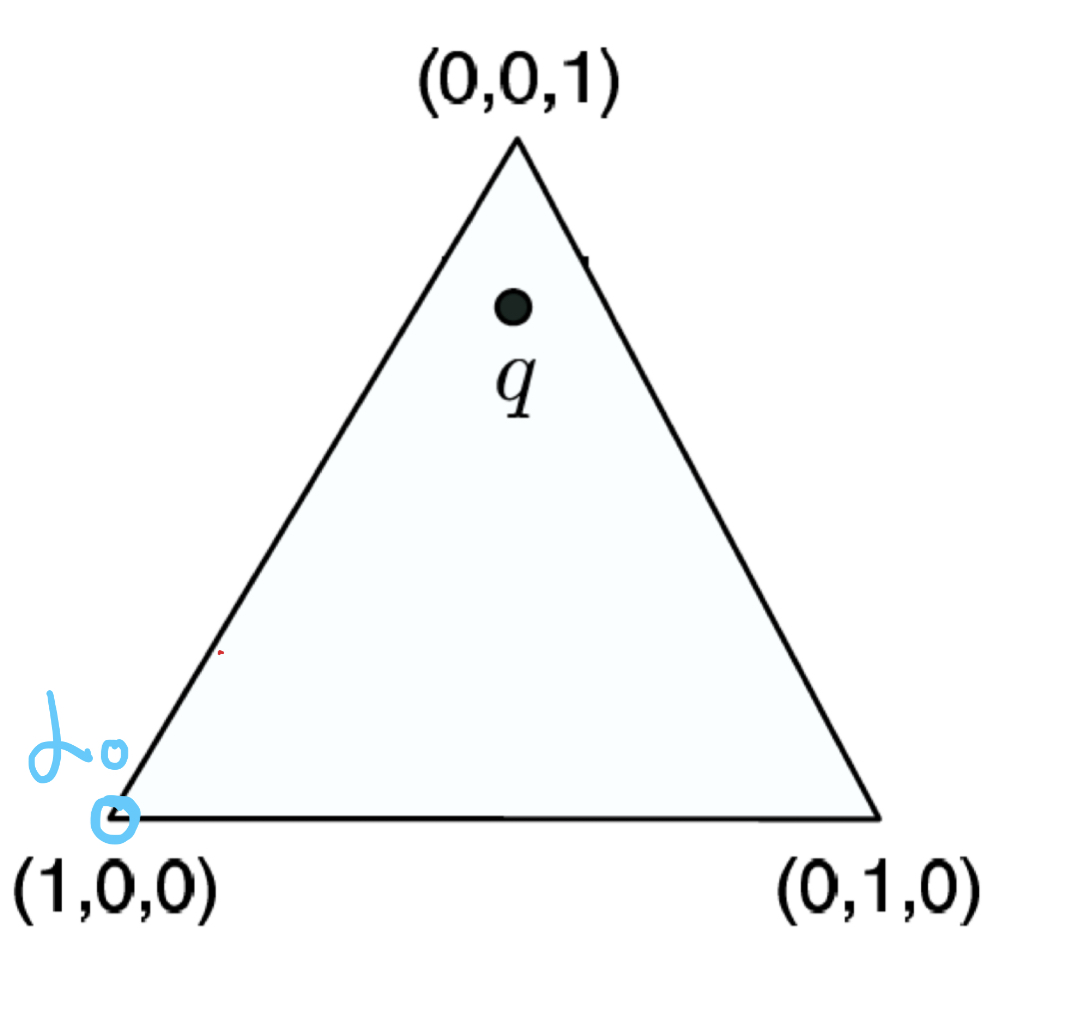
\includegraphics[width = 0.3\linewidth]{3-1.jpg}
    \caption{$\mathcal{L}_0$}
  \end{figure}

  \item $\mathbb{E}_p[\mathrm{y}] = \frac{1}{2}$ means $\mathcal{L}_{\frac{1}{2}} = \left\{p = (p_0,p_1,p_2): p_0+p_1+p_2 = 1,p_1+2p_2 = \frac{1}{2}\right\}$ which is a line passing $(\frac{1}{2},\frac{1}{2},0)$ and $(\frac{3}{4},0,\frac{1}{4})$. 

  \begin{figure}[!htbp]
    \centering
    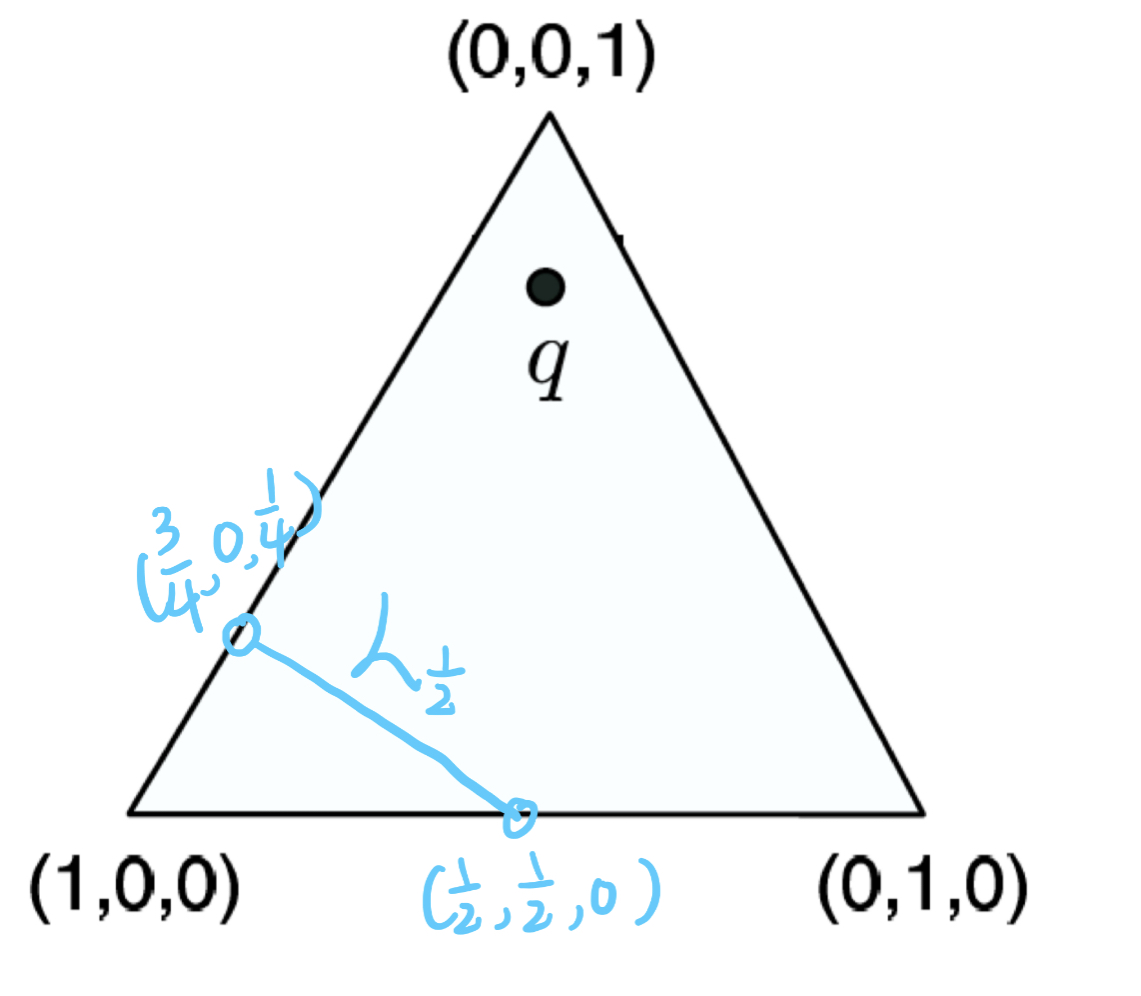
\includegraphics[width = 0.3\linewidth]{3-2.jpg}
    \caption{$\mathcal{L}_{\frac 1 2}$}
  \end{figure}

  \item The exponential family is $\mathcal{E}=\left\{\tilde{q}: \tilde{q}=q e^{s f(\mathrm{y})-\alpha(s)}\right\}$. Following Pythagoras's Identity, let $f(y) = y$ so $\mathcal{E}$ is orthogonal to $\mathcal{L}_{\frac{1}{2}}$.  $\mathcal{E}=\left\{\tilde{q}: \tilde{q}=q e^{s \mathrm{y}-\alpha(s)}\right\}$. Denote $\lambda = e^s$, so $\tilde{q}_0 = \frac{1}{1+\lambda + 4\lambda^2},\tilde{q}_1 = \frac{\lambda}{1+\lambda + 4\lambda^2},\tilde{q}_2 = \frac{4\lambda^2}{1+\lambda + 4\lambda^2}$. Notice that $\mathcal{E}$ passes $(1,0,0)$ and $(0,0,1)$ and $\tilde{q}_1\leqslant \frac{1}{5}$.
  

  \begin{figure}[!htbp]
    \centering
    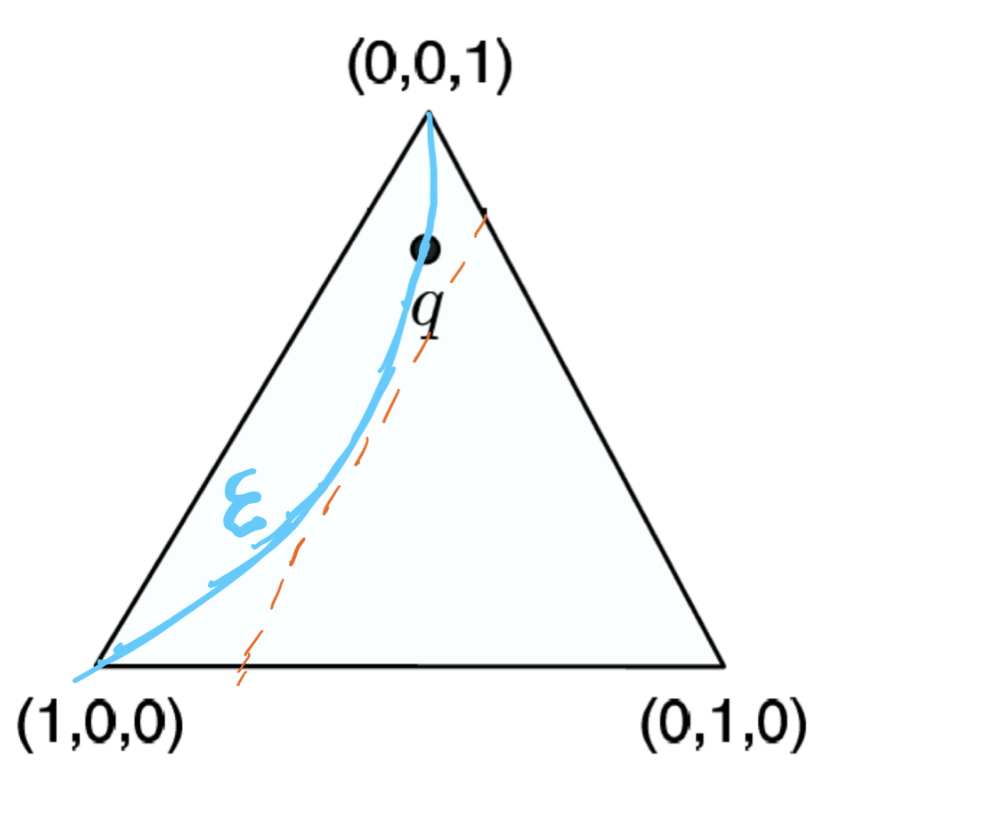
\includegraphics[width = 0.3\linewidth]{3-3.jpg}
    \caption{$\mathcal{E}$}
  \end{figure}

  \item Using the Lagrange-Multiplier method we can induce that the I-projection $p^*$ of $q$ onto $\mathcal{L}_{\frac 1 2}$ belongs to $\mathcal{E}$. So $p^* \in \mathcal{L}_{\frac 1 2} \cap \mathcal{E}$.
  
  \begin{figure}[!htbp]
    \centering
    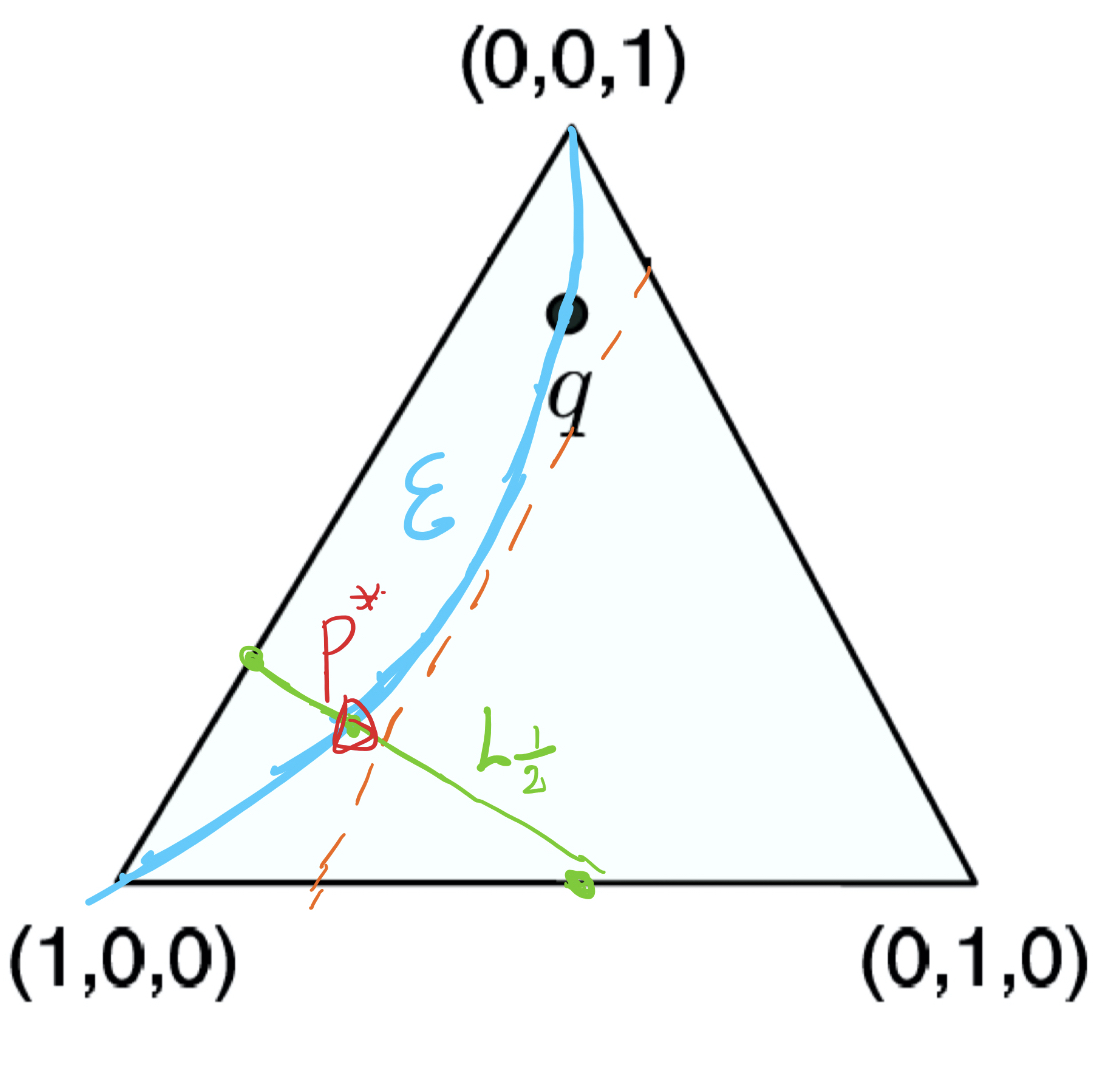
\includegraphics[width = 0.3\linewidth]{3-4.jpg}
    \caption{$p^*$}
  \end{figure}

  By $\tilde{q}_1 + 2 \tilde{q}_2 = \frac{1}{2}$ we can solve $\lambda = \frac{1}{4}$, $p^* = (\frac{2}{3},\frac{1}{6},\frac{1}{6})$ 

  \item As figure \ref{fig:3-5}
  \begin{figure}[!htbp]
    \centering
    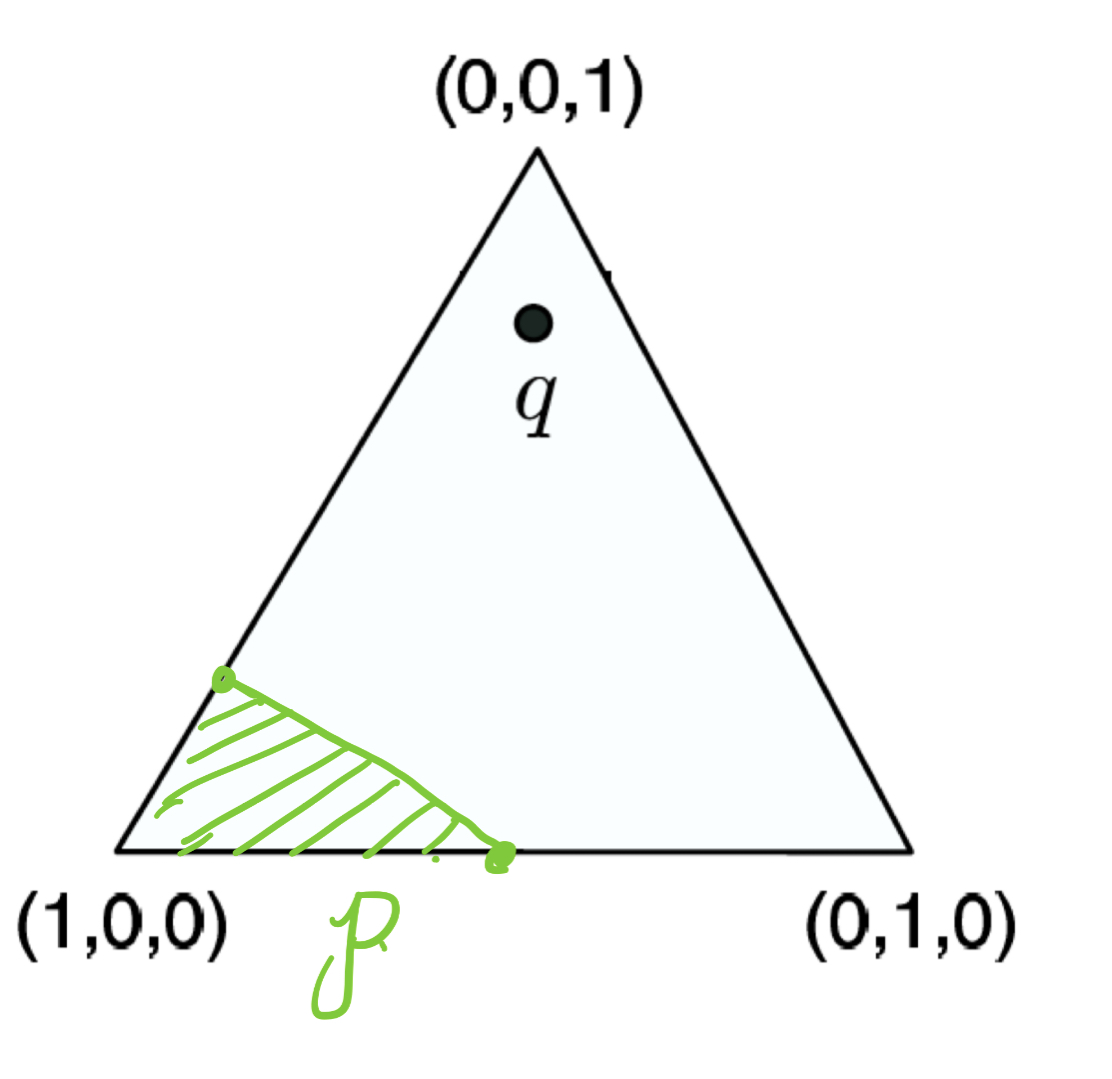
\includegraphics[width = 0.3\linewidth]{3-5.jpg}
    \caption{$\mathcal{P}$}
    \label{fig:3-5}
  \end{figure}

  \item First, for any $p \in \mathcal{P}$, it belongs to some $\mathcal{L}_{\gamma} = {p: \mathbb{E}_p[\mathrm{y}]= \gamma}$ and $\gamma \leqslant \frac{1}{2}$. So $D(p\|q) \geqslant D(p_{\gamma}^* \| q)$ where $p_{\gamma}^*$ is the I-projection of $q$ onto $\mathcal{L}_{\gamma}$. And $p_{\gamma}^* \in \mathcal{E}$. Thus,
  
  \begin{equation}
    p^* = \argmin_{p\in \mathcal{P}} D(p\| q) = \argmin_{p\in \mathcal{P} \cap \mathcal{E}} D(p\| q)
  \end{equation}
  
  For $\tilde{q}_s \in {\mathcal{P} \cap \mathcal{E}}$, $\gamma = \mathbb{E}_{\tilde{q}}[\mathrm{y}] = \tilde{q}_1 + 2 \tilde{q}_2 = \frac{\lambda+8\lambda^2}{1+\lambda+4\lambda^2}, \lambda = e^s$.

  \begin{equation}
    \frac{d\gamma}{d\lambda} = \frac{1+16\lambda+4\lambda^2}{(1+\lambda+4\lambda^2)^2} \geqslant 0
  \end{equation}

  So $\gamma$ strictly increases with $\lambda$, then $\gamma$ strictly increases with $s$, vice versa. And when $\gamma = \frac{1}{2}, \lambda = \frac{1}{4}, s = -\ln 4$

  And $D(\tilde{q}_s \| q) = s \mathbb{E}_{\tilde{q}_s} [ y] - \alpha(s)$.

  \begin{equation}
    \frac{\partial D(\tilde{q}_s \| q)}{\partial s} = s \operatorname{Var}_{\tilde{q}_s} [y] \leqslant 0,\quad \text{for }  s\leqslant -\ln 4 <0
  \end{equation}

  So $\frac{\partial D(\tilde{q}_s \| q)}{\partial \gamma} \leqslant 0$ for $\gamma \leqslant \frac{1}{2}$. To minimize $D(\tilde{q}_s \| q)$, $\gamma^* = \frac{1}{2}, p^* = (\frac{2}{3},\frac{1}{6},\frac{1}{6})$

  \begin{figure}[!htbp]
    \centering
    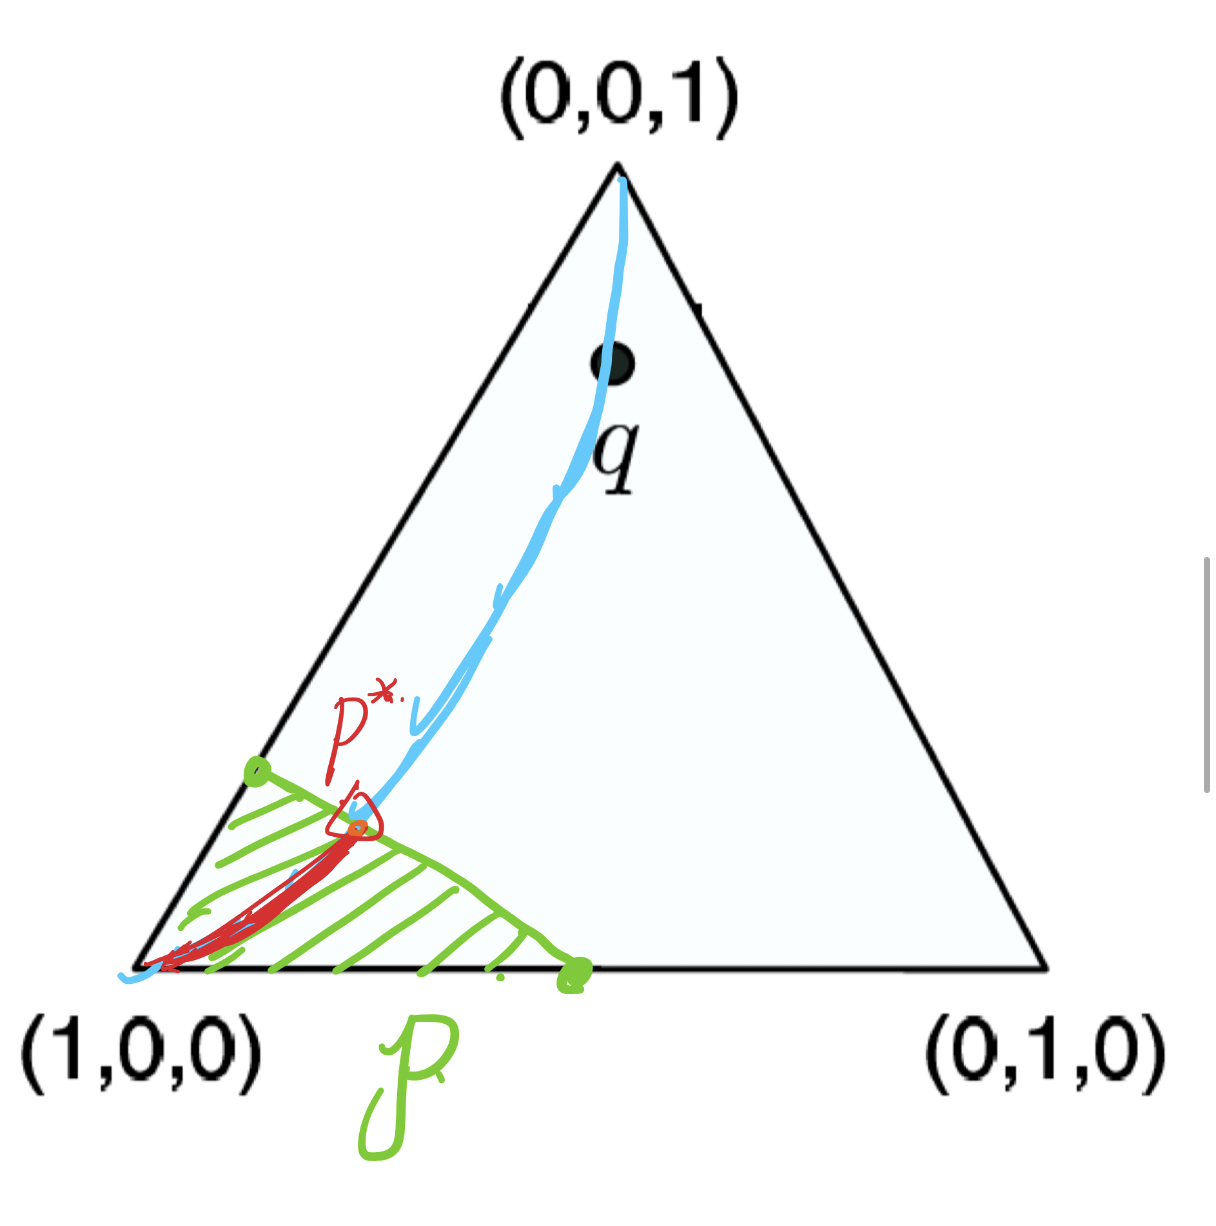
\includegraphics[width = 0.3\linewidth]{3-6.jpg}
    \caption{$p^*$}
    \label{fig:3-6å}
  \end{figure}
\end{enumerate}


\item \begin{enumerate}
  \item $\forall p \in \mathcal{P}$\begin{equation}
    D(q\| p) = \sum_{x=0}^{\infty} q(x) \log \frac{q(x)}{p(x)}
  \end{equation}
  For $x\geqslant M$, $q(x)>0,q(x)=0,q(x) \log \frac{q(x)}{p(x)} = \infty$, so $D(q\| p) = \infty$

  \item $\forall p \in \mathcal{P}$\begin{equation}
    D(p\| q) = \sum_{x=0}^{\infty} p(x) \log \frac{p(x)}{q(x)}
  \end{equation}
  For $x\geqslant M$, $q(x)>0,q(x)=0,p(x) \log \frac{p(x)}{q(x)} = 0$. 
  For $x <M$, $p(x) \log \frac{p(x)}{q(x)} < \infty$, so $D(p\| q) < \infty$

  \item To find the I-projection,\begin{equation}
    \begin{aligned}
      &\min \quad & \sum_{i=0}^{M-1} p_i\log \frac{p_i}{q_i} \\
      &\text{s.t.} \quad & \sum_{i=0}^{M-1} p_i= 1
    \end{aligned}
  \end{equation}

  Using Lagrange Multiplier,

  \begin{equation}
    L = \sum_{i=0}^{M-1} p_i\log \frac{p_i}{q_i}  + \lambda (\sum_{i=0}^{M-1} p_i -1)
  \end{equation}

  \begin{equation}
    \frac{\partial L}{\partial p_i} = 1 + \log \frac{p_i}{q_i}+  \lambda = 0,\quad  i = 0,1,2,\cdot,M-1
  \end{equation}

  So 
  \begin{equation}
    p_i = \frac{q_i}{\sum_{j=0}^{M-1} q_i} = \frac{q_i}{ Q(M-1)}
  \end{equation}

  And

  \begin{equation}
    D(p^*\| q) = \sum_{i=0}^{M-1} p_i\log \frac{p_i}{q_i} = - \log Q(M-1)
  \end{equation}

  \item \begin{equation}
    \begin{aligned}
      &\min \quad & \sum_{i=0}^{\infty} p_i\log \frac{p_i}{q_i} \\
      &\text{s.t.} \quad & \sum_{i=0}^{M-1} p_i= 1-\varepsilon, \\
      &  & \sum_{i=M}^{\infty} p_i= \varepsilon
    \end{aligned}
  \end{equation}

  Using Lagrange Multiplier,

  \begin{equation}
    L = \sum_{i=0}^{\infty} p_i\log \frac{p_i}{q_i}  + \lambda (\sum_{i=0}^{M-1} p_i -1+\varepsilon) + \mu(\sum_{i=M}^{\infty} p_i -\varepsilon)
  \end{equation}

  \begin{equation}
    \begin{aligned}
      &\frac{\partial L}{\partial p_i} = 1 + \log \frac{p_i}{q_i}+  \lambda = 0,\quad  i = 0,1,2,\cdot,M-1 \\
      & \frac{\partial L}{\partial p_i} = 1 + \log \frac{p_i}{q_i}+  \mu = 0,\quad  i = M,\cdot
    \end{aligned}
  \end{equation}

  So \begin{equation}
    p_i = \left\{\begin{aligned}
      &\frac{(1-\varepsilon)q_i}{ Q(M-1)},\quad i = 0,1,2,\cdot,M-1\\
      &\frac{\varepsilon q_i}{ 1-Q(M-1)},\quad i = M,\cdots
    \end{aligned}\right.
  \end{equation}

  And \begin{equation}
    D(p^*_{\varepsilon}\| q) = (1-\varepsilon) \log \frac{1-\varepsilon}{ Q(M-1)} + \varepsilon \log \frac{\varepsilon}{ 1-Q(M-1)}
  \end{equation}

  \begin{equation}
    \lim_{\varepsilon \to 0 }  D(p^*_{\varepsilon}\| q) =  - \log  Q(M-1) = D(p^* \| q)
  \end{equation}

  \item Define a indication function $f(\mathrm{y}) = \mathbf{1}(\mathrm{y} \geqslant M)$, then $\mathcal{P}_{\varepsilon} = \{p: \mathbb{E}_{p}[f(\mathrm{y})] = \epsilon\}$ is a linear family.
  
  \item Because $\mathcal{P}_{\varepsilon}$ is a linear family, the I-projection $p_{\epsilon}^*$ belongs to a exponential family $\mathcal{E} = \{\tilde{q} = qe^{sf(y) - \alpha(s)}\}$. And because $f(y) = \mathbf{1}(\mathrm{y} \geqslant M)$. So $\tilde{q}_i  =  e^{-\alpha(s)} q_i, i =0,1,\cdots,M-1$ and $\tilde{q}_i  =  e^{s-\alpha(s)} q_i, i =M,\cdots$. Comparing with the result in (4), the corresponding parameter \begin{equation}
    s^* = \log \frac{\varepsilon Q(M-1)}{(1-\varepsilon)(1-Q(M-1))}
  \end{equation}
  
\end{enumerate}

\end{enumerate}
  

  
\end{document}
%%% Local Variables:
%%% mode: latex
%%% TeX-master: t
%%% End:
